\documentclass{article}

\usepackage{amsmath,amssymb,amsthm}

\input{macros}
\usepackage{graphics,tikz}
\def\geom{\text{geom}}
\def\sim{\text{sim}}
\def\R{\mathbb{R}}\begin{document}

%FILL IN THE RIGHT INFO.
%\lecture{**LECTURE-NUMBER**}{**DATE**}{**LECTURER**}{**SCRIBE**}
\lecture{8}{Sep 18, 2019}{Don Sheehy}{Palash Gupta, Rishabh Agrawal, Jash Dhakad }

  % \title{Lecture 6}
  % \author{Scribed by: }
  % \maketitle
\section{Handshake Lemma}
\begin{definition}
The number of vertices of odd degree in the graph is even.\\

$\sum\nolimits_{v \in V_G} deg(v) = 2 | E_G|$
 



\section{Tree}
%Let X and Y be simplicial complexes. A simplicial map $f: X \rightarrow Y$ is a pair of functions:
%\centerline {$f_v: V_X \rightarrow V_Y$ and $f_S: S_X \rightarrow S_Y$}

%where $f_S(\sigma) = \{ f_V(u): u \in \sigma \}$
\end{definition}
\begin{theorem}
  Prove that every tree can be drawn in a plane $(R^2 )$  without crossing.
  \end{theorem}
      \begin{proof}[Proof idea]
      
      For any placement of vertices of a tree,we can draw the edges without crossing.To prove this theorem we take an example.Consider the following tree
      
   

\tikzset{every picture/.style={line width=0.75pt}} %set default line width to 0.75pt        

\begin{tikzpicture}[x=0.75pt,y=0.75pt,yscale=-1,xscale=1]
%uncomment if require: \path (0,443.8833312988281); %set diagram left start at 0, and has height of 443.8833312988281

%Shape: Circle [id:dp013251641491293431] 
\draw   (292.23,26.38) .. controls (292.23,15.68) and (300.91,7) .. (311.62,7) .. controls (322.32,7) and (331,15.68) .. (331,26.38) .. controls (331,37.09) and (322.32,45.77) .. (311.62,45.77) .. controls (300.91,45.77) and (292.23,37.09) .. (292.23,26.38) -- cycle ;
%Shape: Circle [id:dp3504718800593517] 
\draw   (95.23,128.38) .. controls (95.23,117.68) and (103.91,109) .. (114.62,109) .. controls (125.32,109) and (134,117.68) .. (134,128.38) .. controls (134,139.09) and (125.32,147.77) .. (114.62,147.77) .. controls (103.91,147.77) and (95.23,139.09) .. (95.23,128.38) -- cycle ;
%Shape: Circle [id:dp6770703678032634] 
\draw   (298.23,133.38) .. controls (298.23,122.68) and (306.91,114) .. (317.62,114) .. controls (328.32,114) and (337,122.68) .. (337,133.38) .. controls (337,144.09) and (328.32,152.77) .. (317.62,152.77) .. controls (306.91,152.77) and (298.23,144.09) .. (298.23,133.38) -- cycle ;
%Shape: Circle [id:dp9905805112353976] 
\draw   (489.23,138.38) .. controls (489.23,127.68) and (497.91,119) .. (508.62,119) .. controls (519.32,119) and (528,127.68) .. (528,138.38) .. controls (528,149.09) and (519.32,157.77) .. (508.62,157.77) .. controls (497.91,157.77) and (489.23,149.09) .. (489.23,138.38) -- cycle ;
%Shape: Circle [id:dp7511891788503602] 
\draw   (38.23,266.38) .. controls (38.23,255.68) and (46.91,247) .. (57.62,247) .. controls (68.32,247) and (77,255.68) .. (77,266.38) .. controls (77,277.09) and (68.32,285.77) .. (57.62,285.77) .. controls (46.91,285.77) and (38.23,277.09) .. (38.23,266.38) -- cycle ;
%Shape: Circle [id:dp4929165659224152] 
\draw   (220.23,270.38) .. controls (220.23,259.68) and (228.91,251) .. (239.62,251) .. controls (250.32,251) and (259,259.68) .. (259,270.38) .. controls (259,281.09) and (250.32,289.77) .. (239.62,289.77) .. controls (228.91,289.77) and (220.23,281.09) .. (220.23,270.38) -- cycle ;
%Shape: Circle [id:dp8063605361374856] 
\draw   (356.23,273.38) .. controls (356.23,262.68) and (364.91,254) .. (375.62,254) .. controls (386.32,254) and (395,262.68) .. (395,273.38) .. controls (395,284.09) and (386.32,292.77) .. (375.62,292.77) .. controls (364.91,292.77) and (356.23,284.09) .. (356.23,273.38) -- cycle ;
%Shape: Circle [id:dp8337477650523604] 
\draw   (444.23,279.38) .. controls (444.23,268.68) and (452.91,260) .. (463.62,260) .. controls (474.32,260) and (483,268.68) .. (483,279.38) .. controls (483,290.09) and (474.32,298.77) .. (463.62,298.77) .. controls (452.91,298.77) and (444.23,290.09) .. (444.23,279.38) -- cycle ;
%Shape: Circle [id:dp3928775345004998] 
\draw   (571.23,283.38) .. controls (571.23,272.68) and (579.91,264) .. (590.62,264) .. controls (601.32,264) and (610,272.68) .. (610,283.38) .. controls (610,294.09) and (601.32,302.77) .. (590.62,302.77) .. controls (579.91,302.77) and (571.23,294.09) .. (571.23,283.38) -- cycle ;
%Shape: Circle [id:dp9093116826516576] 
\draw   (12.23,383.38) .. controls (12.23,372.68) and (20.91,364) .. (31.62,364) .. controls (42.32,364) and (51,372.68) .. (51,383.38) .. controls (51,394.09) and (42.32,402.77) .. (31.62,402.77) .. controls (20.91,402.77) and (12.23,394.09) .. (12.23,383.38) -- cycle ;
%Shape: Circle [id:dp27902713029120785] 
\draw   (108.23,383.38) .. controls (108.23,372.68) and (116.91,364) .. (127.62,364) .. controls (138.32,364) and (147,372.68) .. (147,383.38) .. controls (147,394.09) and (138.32,402.77) .. (127.62,402.77) .. controls (116.91,402.77) and (108.23,394.09) .. (108.23,383.38) -- cycle ;
%Straight Lines [id:da04357009839396775] 
\draw    (126.15,113.95) -- (298.7,41.77) ;


%Straight Lines [id:da8061802219685432] 
\draw    (311.62,45.77) -- (317.62,114) ;


%Straight Lines [id:da3655604140104268] 
\draw    (327,35.95) -- (497,124.95) ;


%Straight Lines [id:da5805838548261475] 
\draw    (114.62,147.77) -- (57.62,247) ;


%Straight Lines [id:da9054176909146017] 
\draw    (239.62,251) -- (317.62,152.77) ;


%Straight Lines [id:da9061864638958759] 
\draw    (317.62,152.77) -- (375.62,254) ;


%Straight Lines [id:da8044378455305757] 
\draw    (463.62,260) -- (508.62,157.77) ;


%Straight Lines [id:da20170981607224014] 
\draw    (508.62,157.77) -- (590.62,264) ;


%Straight Lines [id:da5584656407111704] 
\draw    (57.62,285.77) -- (31.62,364) ;


%Straight Lines [id:da7963986274475852] 
\draw    (57.62,285.77) -- (127.62,364) ;


%Shape: Rectangle [id:dp6756680224361427] 
\draw   (81.75,95.65) -- (557.75,95.65) -- (557.75,175.48) -- (81.75,175.48) -- cycle ;
%Shape: Rectangle [id:dp6176081630971761] 
\draw   (19.75,230.65) -- (641.75,230.65) -- (641.75,305.65) -- (19.75,305.65) -- cycle ;
%Shape: Rectangle [id:dp25213388159487515] 
\draw   (7,355.65) -- (174.75,355.65) -- (174.75,408.65) -- (7,408.65) -- cycle ;

% Text Node
\draw (351,23.48) node  [align=left] {root};


\end{tikzpicture}
 
       
Pick any $v \in V$ to be root. There exists a unique u-v path for all $u \in V$.Assign levels by the length of that path.Another solution is Rooting Graph.  


\tikzset{every picture/.style={line width=0.75pt}} %set default line width to 0.75pt        

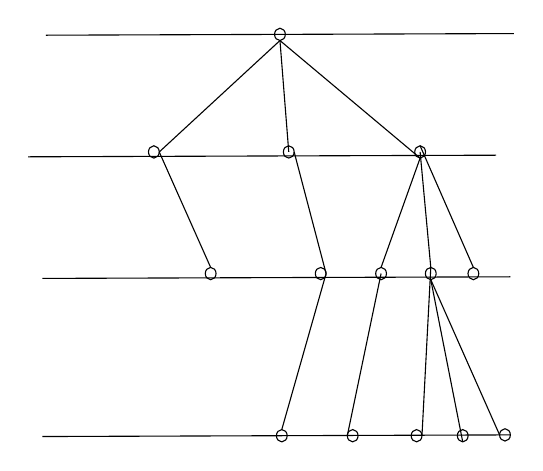
\begin{tikzpicture}[x=0.75pt,y=0.75pt,yscale=-1,xscale=1]
%uncomment if require: \path (0,300); %set diagram left start at 0, and has height of 300

%Straight Lines [id:da8679641386299183] 
\draw    (184.85,42.64) -- (410.3,41.85) ;


%Straight Lines [id:da1823278074000242] 
\draw    (183.14,159.82) -- (408.59,159.04) ;


%Straight Lines [id:da9237788777438267] 
\draw    (176.3,101.23) -- (401.75,100.45) ;


%Straight Lines [id:da15452186287705083] 
\draw    (183.14,236) -- (408.59,235.21) ;


%Shape: Ellipse [id:dp8451771890920043] 
\draw   (294.98,42.25) .. controls (294.98,40.61) and (296.14,39.28) .. (297.58,39.28) .. controls (299.01,39.28) and (300.17,40.61) .. (300.17,42.25) .. controls (300.17,43.88) and (299.01,45.21) .. (297.58,45.21) .. controls (296.14,45.21) and (294.98,43.88) .. (294.98,42.25) -- cycle ;
%Shape: Ellipse [id:dp3605618900924389] 
\draw   (234.23,98.89) .. controls (234.23,97.25) and (235.39,95.92) .. (236.82,95.92) .. controls (238.26,95.92) and (239.42,97.25) .. (239.42,98.89) .. controls (239.42,100.52) and (238.26,101.85) .. (236.82,101.85) .. controls (235.39,101.85) and (234.23,100.52) .. (234.23,98.89) -- cycle ;
%Shape: Ellipse [id:dp011738830314276583] 
\draw   (261.6,157.48) .. controls (261.6,155.84) and (262.76,154.52) .. (264.19,154.52) .. controls (265.63,154.52) and (266.79,155.84) .. (266.79,157.48) .. controls (266.79,159.12) and (265.63,160.44) .. (264.19,160.44) .. controls (262.76,160.44) and (261.6,159.12) .. (261.6,157.48) -- cycle ;
%Shape: Ellipse [id:dp016990569351802765] 
\draw   (314.62,157.48) .. controls (314.62,155.84) and (315.79,154.52) .. (317.22,154.52) .. controls (318.65,154.52) and (319.81,155.84) .. (319.81,157.48) .. controls (319.81,159.12) and (318.65,160.44) .. (317.22,160.44) .. controls (315.79,160.44) and (314.62,159.12) .. (314.62,157.48) -- cycle ;
%Shape: Ellipse [id:dp05248132494427582] 
\draw   (367.65,157.48) .. controls (367.65,155.84) and (368.81,154.52) .. (370.25,154.52) .. controls (371.68,154.52) and (372.84,155.84) .. (372.84,157.48) .. controls (372.84,159.12) and (371.68,160.44) .. (370.25,160.44) .. controls (368.81,160.44) and (367.65,159.12) .. (367.65,157.48) -- cycle ;
%Shape: Ellipse [id:dp4618941899395681] 
\draw   (383.05,235.6) .. controls (383.05,233.97) and (384.21,232.64) .. (385.64,232.64) .. controls (387.07,232.64) and (388.23,233.97) .. (388.23,235.6) .. controls (388.23,237.24) and (387.07,238.57) .. (385.64,238.57) .. controls (384.21,238.57) and (383.05,237.24) .. (383.05,235.6) -- cycle ;
%Shape: Ellipse [id:dp48843211369986905] 
\draw   (388.18,157.48) .. controls (388.18,155.84) and (389.34,154.52) .. (390.77,154.52) .. controls (392.2,154.52) and (393.37,155.84) .. (393.37,157.48) .. controls (393.37,159.12) and (392.2,160.44) .. (390.77,160.44) .. controls (389.34,160.44) and (388.18,159.12) .. (388.18,157.48) -- cycle ;
%Shape: Ellipse [id:dp5262182698248602] 
\draw   (299.23,98.89) .. controls (299.23,97.25) and (300.39,95.92) .. (301.82,95.92) .. controls (303.26,95.92) and (304.42,97.25) .. (304.42,98.89) .. controls (304.42,100.52) and (303.26,101.85) .. (301.82,101.85) .. controls (300.39,101.85) and (299.23,100.52) .. (299.23,98.89) -- cycle ;
%Shape: Ellipse [id:dp60762823657962] 
\draw   (360.81,235.6) .. controls (360.81,233.97) and (361.97,232.64) .. (363.4,232.64) .. controls (364.84,232.64) and (366,233.97) .. (366,235.6) .. controls (366,237.24) and (364.84,238.57) .. (363.4,238.57) .. controls (361.97,238.57) and (360.81,237.24) .. (360.81,235.6) -- cycle ;
%Shape: Ellipse [id:dp005588247345829078] 
\draw   (343.7,157.48) .. controls (343.7,155.84) and (344.87,154.52) .. (346.3,154.52) .. controls (347.73,154.52) and (348.89,155.84) .. (348.89,157.48) .. controls (348.89,159.12) and (347.73,160.44) .. (346.3,160.44) .. controls (344.87,160.44) and (343.7,159.12) .. (343.7,157.48) -- cycle ;
%Shape: Ellipse [id:dp8196914442684315] 
\draw   (362.52,98.89) .. controls (362.52,97.25) and (363.68,95.92) .. (365.11,95.92) .. controls (366.55,95.92) and (367.71,97.25) .. (367.71,98.89) .. controls (367.71,100.52) and (366.55,101.85) .. (365.11,101.85) .. controls (363.68,101.85) and (362.52,100.52) .. (362.52,98.89) -- cycle ;
%Shape: Ellipse [id:dp6919024995083671] 
\draw   (295.87,235.6) .. controls (295.87,233.97) and (297.03,232.64) .. (298.46,232.64) .. controls (299.89,232.64) and (301.05,233.97) .. (301.05,235.6) .. controls (301.05,237.24) and (299.89,238.57) .. (298.46,238.57) .. controls (297.03,238.57) and (295.87,237.24) .. (295.87,235.6) -- cycle ;
%Shape: Ellipse [id:dp9396365309919391] 
\draw   (330.02,235.6) .. controls (330.02,233.97) and (331.18,232.64) .. (332.61,232.64) .. controls (334.05,232.64) and (335.21,233.97) .. (335.21,235.6) .. controls (335.21,237.24) and (334.05,238.57) .. (332.61,238.57) .. controls (331.18,238.57) and (330.02,237.24) .. (330.02,235.6) -- cycle ;
%Shape: Ellipse [id:dp009053637437229534] 
\draw   (403.4,235.21) .. controls (403.4,233.58) and (404.56,232.25) .. (406,232.25) .. controls (407.43,232.25) and (408.59,233.58) .. (408.59,235.21) .. controls (408.59,236.85) and (407.43,238.18) .. (406,238.18) .. controls (404.56,238.18) and (403.4,236.85) .. (403.4,235.21) -- cycle ;
%Straight Lines [id:da44184321284323913] 
\draw    (297.58,45.21) -- (239.42,98.89) ;


%Straight Lines [id:da21669874790911836] 
\draw    (297.58,45.21) -- (301.82,98.89) ;


%Straight Lines [id:da45537103314486427] 
\draw    (297.58,45.21) -- (365.11,101.85) ;


%Straight Lines [id:da44156620034838145] 
\draw    (239.42,98.89) -- (264.19,154.52) ;


%Straight Lines [id:da24037049620640927] 
\draw    (304.42,98.89) -- (319.81,157.48) ;


%Straight Lines [id:da0302570993886776] 
\draw    (365.11,101.85) -- (346.3,154.52) ;


%Straight Lines [id:da6370870438774625] 
\draw    (365.11,98.89) -- (370.25,154.52) ;


%Straight Lines [id:da10986501157735229] 
\draw    (365.11,95.92) -- (390.77,154.52) ;


%Straight Lines [id:da8402963105985113] 
\draw    (370.25,160.44) -- (403.4,235.21) ;


%Straight Lines [id:da7833025415255381] 
\draw    (370.25,154.52) -- (366,235.6) ;


%Straight Lines [id:da9340919497733094] 
\draw    (370.25,160.44) -- (385.64,238.57) ;


%Straight Lines [id:da0344499106711873] 
\draw    (346.3,157.48) -- (330.02,235.6) ;


%Straight Lines [id:da6165594303193094] 
\draw    (319.81,157.48) -- (298.46,232.64) ;






\end{tikzpicture}


\
  
\begin{theorem}
Every binary tree has at least one edge edge (u,v) such that G \textbackslash(u,v) has 2 components and neither has more than (2n)/3 vertices.
\end{theorem}
\begin{proof}[Proof idea]



\tikzset{every picture/.style={line width=0.75pt}} %set default line width to 0.75pt        

\begin{tikzpicture}[x=0.75pt,y=0.75pt,yscale=-1,xscale=1]
%uncomment if require: \path (0,300); %set diagram left start at 0, and has height of 300

%Shape: Ellipse [id:dp5026941740532689] 
\draw   (263.97,36.47) .. controls (263.97,32.41) and (268.66,29.12) .. (274.45,29.12) .. controls (280.23,29.12) and (284.92,32.41) .. (284.92,36.47) .. controls (284.92,40.52) and (280.23,43.81) .. (274.45,43.81) .. controls (268.66,43.81) and (263.97,40.52) .. (263.97,36.47) -- cycle ;
%Shape: Ellipse [id:dp8052290539693855] 
\draw   (248.82,108.6) .. controls (248.82,104.55) and (253.52,101.25) .. (259.3,101.25) .. controls (265.09,101.25) and (269.78,104.55) .. (269.78,108.6) .. controls (269.78,112.66) and (265.09,115.95) .. (259.3,115.95) .. controls (253.52,115.95) and (248.82,112.66) .. (248.82,108.6) -- cycle ;
%Shape: Ellipse [id:dp5260936609004553] 
\draw   (158.75,106.93) .. controls (158.75,102.87) and (163.44,99.58) .. (169.23,99.58) .. controls (175.01,99.58) and (179.7,102.87) .. (179.7,106.93) .. controls (179.7,110.98) and (175.01,114.28) .. (169.23,114.28) .. controls (163.44,114.28) and (158.75,110.98) .. (158.75,106.93) -- cycle ;
%Shape: Ellipse [id:dp0005502308215511453] 
\draw   (302.23,66.1) .. controls (302.23,62.05) and (306.92,58.75) .. (312.71,58.75) .. controls (318.49,58.75) and (323.18,62.05) .. (323.18,66.1) .. controls (323.18,70.16) and (318.49,73.45) .. (312.71,73.45) .. controls (306.92,73.45) and (302.23,70.16) .. (302.23,66.1) -- cycle ;
%Shape: Ellipse [id:dp49902676693437586] 
\draw   (209.77,65.54) .. controls (209.77,61.49) and (214.46,58.2) .. (220.24,58.2) .. controls (226.03,58.2) and (230.72,61.49) .. (230.72,65.54) .. controls (230.72,69.6) and (226.03,72.89) .. (220.24,72.89) .. controls (214.46,72.89) and (209.77,69.6) .. (209.77,65.54) -- cycle ;
%Straight Lines [id:da189102538082779] 
\draw    (274.45,43.81) -- (220.24,58.2) ;


%Straight Lines [id:da8842093294465067] 
\draw    (274.45,43.81) -- (312.71,58.75) ;


%Straight Lines [id:da3777940096483836] 
\draw    (169.23,99.58) -- (220.24,72.89) ;


%Straight Lines [id:da8028300693428679] 
\draw    (259.3,101.25) -- (220.24,72.89) ;


%Shape: Ellipse [id:dp65926601971189] 
\draw   (191.97,232.47) .. controls (191.97,228.41) and (196.66,225.12) .. (202.45,225.12) .. controls (208.23,225.12) and (212.92,228.41) .. (212.92,232.47) .. controls (212.92,236.52) and (208.23,239.81) .. (202.45,239.81) .. controls (196.66,239.81) and (191.97,236.52) .. (191.97,232.47) -- cycle ;
%Shape: Ellipse [id:dp6411355252121014] 
\draw   (109.97,231.47) .. controls (109.97,227.41) and (114.66,224.12) .. (120.45,224.12) .. controls (126.23,224.12) and (130.92,227.41) .. (130.92,231.47) .. controls (130.92,235.52) and (126.23,238.81) .. (120.45,238.81) .. controls (114.66,238.81) and (109.97,235.52) .. (109.97,231.47) -- cycle ;
%Straight Lines [id:da5016048102790736] 
\draw    (165.12,193.65) -- (153.12,202.65) ;


%Straight Lines [id:da9396382704817337] 
\draw    (148.12,205.65) -- (136.12,214.65) ;


%Straight Lines [id:da5266599741439887] 
\draw    (132.45,215.12) -- (120.45,224.12) ;


%Straight Lines [id:da8645457315504854] 
\draw    (169.22,196.65) -- (183.22,208.65) ;


%Straight Lines [id:da5660632425660811] 
\draw    (187.22,212.65) -- (202.45,225.12) ;


%Shape: Circle [id:dp8947826209460452] 
\draw   (377.52,234.87) .. controls (377.52,229.48) and (381.89,225.1) .. (387.29,225.1) .. controls (392.69,225.1) and (397.07,229.48) .. (397.07,234.87) .. controls (397.07,240.27) and (392.69,244.65) .. (387.29,244.65) .. controls (381.89,244.65) and (377.52,240.27) .. (377.52,234.87) -- cycle ;
%Shape: Circle [id:dp7757098827760354] 
\draw   (415.52,284.87) .. controls (415.52,279.48) and (419.89,275.1) .. (425.29,275.1) .. controls (430.69,275.1) and (435.07,279.48) .. (435.07,284.87) .. controls (435.07,290.27) and (430.69,294.65) .. (425.29,294.65) .. controls (419.89,294.65) and (415.52,290.27) .. (415.52,284.87) -- cycle ;
%Shape: Circle [id:dp5978185823414772] 
\draw   (329.52,284.87) .. controls (329.52,279.48) and (333.89,275.1) .. (339.29,275.1) .. controls (344.69,275.1) and (349.07,279.48) .. (349.07,284.87) .. controls (349.07,290.27) and (344.69,294.65) .. (339.29,294.65) .. controls (333.89,294.65) and (329.52,290.27) .. (329.52,284.87) -- cycle ;
%Straight Lines [id:da544800641882542] 
\draw    (387.29,244.65) -- (339.29,275.1) ;


%Straight Lines [id:da0421722164760574] 
\draw    (387.29,244.65) -- (425.29,275.1) ;



% Text Node
\draw (274.45,36.47) node  [align=left] {n};
% Text Node
\draw (220.24,65.54) node  [align=left] {?};
% Text Node
\draw (312.71,66.1) node  [align=left] {?};
% Text Node
\draw (169.23,106.93) node  [align=left] {?};
% Text Node
\draw (259.3,108.6) node  [align=left] {?};
% Text Node
\draw (170.14,146.17) node  [align=left] {..\\...\\\\..\\..};
% Text Node
\draw (120.45,231.47) node  [align=left] {1};
% Text Node
\draw (202.45,232.47) node  [align=left] {1};
% Text Node
\draw (283.13,232.93) node  [align=left] {else somewhere };
% Text Node
\draw (419.07,234.1) node  [align=left] {> 2n/3};
% Text Node
\draw (303.03,285.17) node  [align=left] {< n/3};
% Text Node
\draw (459.03,285) node  [align=left] {< n/3};


\end{tikzpicture}

\end{proof}


\section{Outer Planar Graph}
\begin{definition}
A graph is outer planar if it can be embedded in the plane so that every vertex is on the same face.

$G \rightarrow geom (G) \subseteq {R^n}$\xrightarrow[\text{}]{\text{embed}}$Embedding \subseteq {R^2}$

The second mapping (the embed one) is an injective mapping.

\end{definition}



\begin{definition}
Faces of $\underbar{G}$ are path connected components of ${R^2}$\textbackslash\underbar{G} 
\end{definition}

Some examples are


\tikzset{every picture/.style={line width=0.75pt}} %set default line width to 0.75pt        

\begin{tikzpicture}[x=0.75pt,y=0.75pt,yscale=-1,xscale=1]
%uncomment if require: \path (0,300); %set diagram left start at 0, and has height of 300

%Flowchart: Decision [id:dp8888176421485359] 
\draw   (199.56,94.7) -- (273.21,141.58) -- (199.56,188.46) -- (125.9,141.58) -- cycle ;
%Shape: Ellipse [id:dp6760978318532891] 
\draw   (198.47,95.91) .. controls (198.47,95.24) and (198.96,94.7) .. (199.56,94.7) .. controls (200.16,94.7) and (200.64,95.24) .. (200.64,95.91) .. controls (200.64,96.58) and (200.16,97.12) .. (199.56,97.12) .. controls (198.96,97.12) and (198.47,96.58) .. (198.47,95.91) -- cycle ;
%Shape: Ellipse [id:dp2329693039703622] 
\draw   (197.38,188.46) .. controls (197.38,187.79) and (197.87,187.24) .. (198.47,187.24) .. controls (199.07,187.24) and (199.56,187.79) .. (199.56,188.46) .. controls (199.56,189.12) and (199.07,189.67) .. (198.47,189.67) .. controls (197.87,189.67) and (197.38,189.12) .. (197.38,188.46) -- cycle ;
%Shape: Ellipse [id:dp81170310784359] 
\draw   (272.13,140.37) .. controls (272.13,139.7) and (272.61,139.16) .. (273.21,139.16) .. controls (273.81,139.16) and (274.3,139.7) .. (274.3,140.37) .. controls (274.3,141.04) and (273.81,141.58) .. (273.21,141.58) .. controls (272.61,141.58) and (272.13,141.04) .. (272.13,140.37) -- cycle ;
%Shape: Ellipse [id:dp6595798796647364] 
\draw   (125.9,141.58) .. controls (125.9,140.91) and (126.39,140.37) .. (126.99,140.37) .. controls (127.59,140.37) and (128.07,140.91) .. (128.07,141.58) .. controls (128.07,142.25) and (127.59,142.79) .. (126.99,142.79) .. controls (126.39,142.79) and (125.9,142.25) .. (125.9,141.58) -- cycle ;

% Text Node
\draw (322,138.32) node  [align=left] {};
% Text Node
\draw (120,180.32) node   {$$};


\end{tikzpicture}
 

\tikzset{every picture/.style={line width=0.75pt}} %set default line width to 0.75pt        

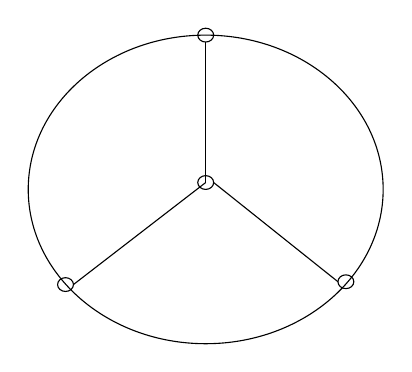
\begin{tikzpicture}[x=0.75pt,y=0.75pt,yscale=-1,xscale=1]
%uncomment if require: \path (0,300); %set diagram left start at 0, and has height of 300

%Shape: Ellipse [id:dp13065196607854535] 
\draw   (186.38,164.26) .. controls (186.38,123.21) and (224.66,89.92) .. (271.88,89.92) .. controls (319.1,89.92) and (357.38,123.21) .. (357.38,164.26) .. controls (357.38,205.32) and (319.1,238.6) .. (271.88,238.6) .. controls (224.66,238.6) and (186.38,205.32) .. (186.38,164.26) -- cycle ;
%Shape: Ellipse [id:dp803169309486954] 
\draw   (268.06,89.92) .. controls (268.06,88.09) and (269.77,86.6) .. (271.88,86.6) .. controls (273.99,86.6) and (275.71,88.09) .. (275.71,89.92) .. controls (275.71,91.76) and (273.99,93.25) .. (271.88,93.25) .. controls (269.77,93.25) and (268.06,91.76) .. (268.06,89.92) -- cycle ;
%Shape: Ellipse [id:dp7844010278319313] 
\draw   (268.06,160.94) .. controls (268.06,159.1) and (269.77,157.62) .. (271.88,157.62) .. controls (273.99,157.62) and (275.71,159.1) .. (275.71,160.94) .. controls (275.71,162.77) and (273.99,164.26) .. (271.88,164.26) .. controls (269.77,164.26) and (268.06,162.77) .. (268.06,160.94) -- cycle ;
%Shape: Ellipse [id:dp9725021620461569] 
\draw   (335.6,208.74) .. controls (335.6,206.9) and (337.31,205.41) .. (339.42,205.41) .. controls (341.54,205.41) and (343.25,206.9) .. (343.25,208.74) .. controls (343.25,210.57) and (341.54,212.06) .. (339.42,212.06) .. controls (337.31,212.06) and (335.6,210.57) .. (335.6,208.74) -- cycle ;
%Shape: Ellipse [id:dp8074058938003839] 
\draw   (200.52,210.1) .. controls (200.52,208.27) and (202.23,206.78) .. (204.34,206.78) .. controls (206.45,206.78) and (208.16,208.27) .. (208.16,210.1) .. controls (208.16,211.94) and (206.45,213.43) .. (204.34,213.43) .. controls (202.23,213.43) and (200.52,211.94) .. (200.52,210.1) -- cycle ;
%Straight Lines [id:da898486259474777] 
\draw    (271.88,93.25) -- (271.88,160.94) ;


%Straight Lines [id:da49964080934779065] 
\draw    (271.88,160.94) -- (208.16,210.1) ;


%Straight Lines [id:da6001366942647658] 
\draw    (275.71,160.94) -- (335.6,208.74) ;






\end{tikzpicture}
${K_4}$



\tikzset{every picture/.style={line width=0.75pt}} %set default line width to 0.75pt        

\begin{tikzpicture}[x=0.75pt,y=0.75pt,yscale=-1,xscale=1]
%uncomment if require: \path (0,284.9499969482422); %set diagram left start at 0, and has height of 284.9499969482422

%Shape: Circle [id:dp4341599909097572] 
\draw   (208.15,138.72) .. controls (208.15,85.63) and (251.18,42.6) .. (304.27,42.6) .. controls (357.35,42.6) and (400.38,85.63) .. (400.38,138.72) .. controls (400.38,191.8) and (357.35,234.83) .. (304.27,234.83) .. controls (251.18,234.83) and (208.15,191.8) .. (208.15,138.72) -- cycle ;
%Shape: Circle [id:dp05031934125487825] 
\draw   (301.65,42.6) .. controls (301.65,41.15) and (302.82,39.98) .. (304.27,39.98) .. controls (305.71,39.98) and (306.88,41.15) .. (306.88,42.6) .. controls (306.88,44.05) and (305.71,45.22) .. (304.27,45.22) .. controls (302.82,45.22) and (301.65,44.05) .. (301.65,42.6) -- cycle ;
%Shape: Circle [id:dp6917794558042587] 
\draw   (310.65,234.6) .. controls (310.65,233.15) and (311.82,231.98) .. (313.27,231.98) .. controls (314.71,231.98) and (315.88,233.15) .. (315.88,234.6) .. controls (315.88,236.05) and (314.71,237.22) .. (313.27,237.22) .. controls (311.82,237.22) and (310.65,236.05) .. (310.65,234.6) -- cycle ;
%Shape: Circle [id:dp8624475773980107] 
\draw   (205.53,136.1) .. controls (205.53,134.65) and (206.7,133.48) .. (208.15,133.48) .. controls (209.6,133.48) and (210.77,134.65) .. (210.77,136.1) .. controls (210.77,137.55) and (209.6,138.72) .. (208.15,138.72) .. controls (206.7,138.72) and (205.53,137.55) .. (205.53,136.1) -- cycle ;
%Shape: Circle [id:dp6691645345701613] 
\draw   (397.77,136.1) .. controls (397.77,134.65) and (398.94,133.48) .. (400.38,133.48) .. controls (401.83,133.48) and (403,134.65) .. (403,136.1) .. controls (403,137.55) and (401.83,138.72) .. (400.38,138.72) .. controls (398.94,138.72) and (397.77,137.55) .. (397.77,136.1) -- cycle ;
%Straight Lines [id:da04640618655790518] 
\draw    (210.77,136.1) -- (306.38,136.1) -- (397.77,136.1) ;


%Shape: Circle [id:dp2782395878542163] 
\draw   (301.65,136.1) .. controls (301.65,134.65) and (302.82,133.48) .. (304.27,133.48) .. controls (305.71,133.48) and (306.88,134.65) .. (306.88,136.1) .. controls (306.88,137.55) and (305.71,138.72) .. (304.27,138.72) .. controls (302.82,138.72) and (301.65,137.55) .. (301.65,136.1) -- cycle ;




\end{tikzpicture}
${K_2,3}$

Note:
If a Graph G does not have a minor M,then its contraction G' also does not have a minor.
\end{document}